%!TEX root = document.tex

Now we analyse the informativeness of Activity Social Affinity
Features (ASAFs) by looking at the correlation between the size and
type of groups, pages and favourites.

Fig~\ref{Fig3} provides scatter plots of conditional
entropies and logistic regression weights vs. activity group 
size.\footnote{Here the size of a {\em group}, {\em page} and {\em favourite}
is the number of total users in the activity group.  For {\em pages}
and {\em favorites} this is the total number of Facebook users,
whether or not they are in the App users' ego network, while for {\em
groups} only the number of users in the App users' ego network is
visible to our App.}  Both plots show that small activity groups
\emph{can} be highly predictive (low conditional entropy or
weights that deviate extremely from zero) whereas large groups are
\emph{rarely} predictive.

In Fig~\ref{Fig4} we plot the average conditional entropy of the top
10\% of features cumulative up to the size of the activity group given
on the x-axis.
%; this allows us to determine the marginal contribution
%of larger groups to the average conditional entropy as they 
%are incrementally added in.  
This graph distinctly shows that the
small sizes of groups, pages and favourites have low average
conditional entropy that transitions sharply to a higher average 
at about 50 for groups and $10^{5}$ for pages/favourites.

We also analyse predictiveness of favourites by categories obtained
from the Facebook API in Fig~\ref{Fig5}.  While half of category
instances in movie, books, or movies with ``long-tail'' (less popular,
specialised) content may not be highly predictive (judging by median
informativess), these categories do contain some highly predictive
instances (as evidenced by the top two quartiles).  On the contrary,
highly generic categories (e.g. interests) and those with fewer
choices (e.g. sports or fav-teams) tend to be less predictive overall.
These observations of Fig~\ref{Fig5} are also reiterated by the
examples provided in Table~\ref{table:fav_examples} where
uninformative favourites tend to have a broad appeal whereas
informative favourites generally appear much more specialised.  This
reinforces the insight of SAF that it is important to learn
which SAGs are predictive.
   
%#suvash#
One might ask how the number of activities a user joins affects
recommendation performance.  In Fig~\ref{AccuracyVsmembership}, we see
that on average, more user activities generally leads to higher
accuracy.  As an alternative analysis, Fig~\ref{fig:features_overview}
shows performance vs.  the number of \emph{active features}, i.e., for
any (user,item) recommendation in a row of
Fig~\ref{fig:features_overview}, the active features are those that
are true (1).  Here we see that excessive item popularity among
activities hurts the discriminative power of SAF to make good
recommendations.

\begin{table*}[t!] \centering 

{\small
\begin{tabular}{|c|c|c|c|c|}
\hline 
\multicolumn{5}{|c|}{\textbf{Median Informative Favourites by Category}}\\
\hline 
\textbf{Books} & \textbf{Movies} & \textbf{Music} & \textbf{Television} & \textbf{Interests} \\
\hline \hline
Harry Potter series&Forrest Gump&John Lennon&Futurama&Travel\\
\hline
A Song of Ice and Fire&Pretty Woman&U2&Star Trek&Music\\
\hline
Discworld&Napoleon Dynamite&AC/DC&The Trap Door&Literature\\
\hline
Hitchhiker's Guide To The Galaxy&Harry Potter&The Smashing Pumpkins&Drawn Together&Painting\\
\hline
The Hobbit&Toy Story 3&Gotye&Sherlock(Official)&Running\\
\hline
The Magician's Guild&The Godfather&The Rolling Stones&Hitchhiker's Guide to the Galaxy&Sports\\
\hline
Ranger's Apprentice&Mulan&All Axess&Buffy The Vampire Slayer&Films\\
\hline
Cosmos&How to Train Your Dragon&Steve Aoki&South Park&Genetics\\
\hline
%Foundation and Earth&The Princess Bride&Rihanna&24&Travelling\\
%\hline
%Deception Point&Watchmen&Billy Joel&The Daily Show&Internet\\
%\hline
%%%%%%
%5 point someone&Black Swan&Queens of the Stone Age&Monty Python's Flying Circus&Psychology\\
%\hline
%Freakonomics&Inception&Depeche Mode&Top Chef&Math\\
%\hline
%Alex Rider Series&Donnie Darko&Oasis&The Inbetweeners&Lambda\\
%\hline
%The Elenium&Kung Fu Panda&Justice&Firefly&Computer Science\\
%\hline
%Watchmen&American Psycho&Gorillaz&Red Dwarf&Skepticism\\
%\hline
\multicolumn{5}{c}{}\\
\hline 
\multicolumn{5}{|c|}{\textbf{Most Informative Favourites by Category}}\\
\hline
\textbf{Books} & \textbf{Movies} & \textbf{Music} & \textbf{Television} & \textbf{Interests} \\
\hline \hline
Calvin and Hobbes & Billy Madison & Avascular Necrosis & Metalocalypse & Computers\\
\hline
Tomorrow when the War Began & Team America: World Police & Tortured & Beast Wars & Texas HoldEm \\
\hline
I really like ceilings  & Pan's Labyrinth & Elysian & Hey Arnold! & Programming\\
\hline
Angels and demons  & Pirates of the Caribbean & Anno Domini & Sherlock & Economics\\
\hline
Magician  & Aladdin & Darker Half & Hey Hey It's Saturday & Martial arts\\
\hline
Digital Fortress  & Starship Troopers & Hellbringer & Neil Buchanan and Art Attack! & Graphic design\\
\hline
The Bible  & Happy Gilmore & Johnny Roadkill & Breaking Bad & Cooking\\
\hline
Interview with the Vampire  & Timon and Pumbaa & Aeon of Horus & Red vs. Blue & Klingon language\\
\hline
%The Discworld Series  & Ferris Buellers Day Off & Katabasis & Stargate Universe & Politics\\
%\hline
%The Da Vinci Code  & Peter Griffin & Bane Of Isildur & Chaser's War on Everything & Science\\
%\hline
\end{tabular}}

\caption{(top) Examples of 8 items per Favourite category near the \emph{median} conditional entropy (\emph{median informativeness}).
(bottom) Examples of top 8 items with the lowest conditional entropy
(\emph{most informative}).  A general trend is that more informative
favourite category ASAGs tend to be more specialised in appeal,
e.g. ``Avascular Necrosis'' is an informative music group favourite
--- its members tend to share common preferences --- while ``John
Lennon'' and ``U2'' have a broader audience with more diverse
preferences.
%#suvash#
Interestingly, ''Sherlock'' appears in both most and median
informative table but the median informative is an official page with
wide range of fans, whereas the most informative is a duplicate fan
page with few fans.}
\label{table:fav_examples}
\end{table*}

\eat{
\begin{table*}[tbp!]
\centering
\begin{tabular}{| >{\small}l | >{\small}r | >{\small}r |}
\hline
\textbf{Top Groups} & \textbf{Top Pages} & \textbf{Top Favourites} \\
\hline
%Heavy Metal - Australian Capital Territory & Avascular Necrosis & Avascular Necrosis \\
Heavy Metal - (city name) & Avascular Necrosis & Avascular Necrosis \\
Stephen Conroy Should Not Filter Our Internet & Assidian & Tortured \\
Silicone Stripper & Tortured & Elysian \\
Hardcore dancing is not moshing & Elysian & Anno Domini \\
%Metal bands come to Canberra cause I'm sick of... & Darker Half & Hellbringer \\
Metal bands come to (city name) cause I'm sick of... & Darker Half & Hellbringer \\
%Canberra Rock Gigs & Johnny Roadkill & Johnny Roadkill \\
(city name) Rock Gigs & Johnny Roadkill & Johnny Roadkill \\
%Let's Mosh - Canberra metal radio show - 2XX 9 & Anno Domini & Darker Half \\
Let's Mosh - (city name) metal radio show - 2XX 9 & Anno Domini & Darker Half \\
Bring Steel Panther to Australia & Billy Madison & Bane Of Isildur \\
%Canberra Death/Heavy Metal Appreciation & Hellbringer & Katabasis \\
(city name)  Death/Heavy Metal Appreciation & Hellbringer & Katabasis \\
Robert The Bruce (Band) & Metalocalypse & Aeon of Horus \\
\hline
\end{tabular}
\caption{Top 10 Groups/Pages/Favourites ranked by Conditional Entropy. The city name where our institution and many Facebook users resides is anonymized.}
\label {table:topGroupPagesFavs}
\end{table*}}

%%%%%%%%%%%%%%%%%%%%%%%%%%%%%%%%%%%%%%%%%%%%%%%%%%%%%%%%%%%%%%%%%%%%%%%%%%%
\begin{figure*}[tbph!]
\centering
\begin{tabular}{ccc}
\begin{tabular}{ccc}
\subfloat[Fig:][]{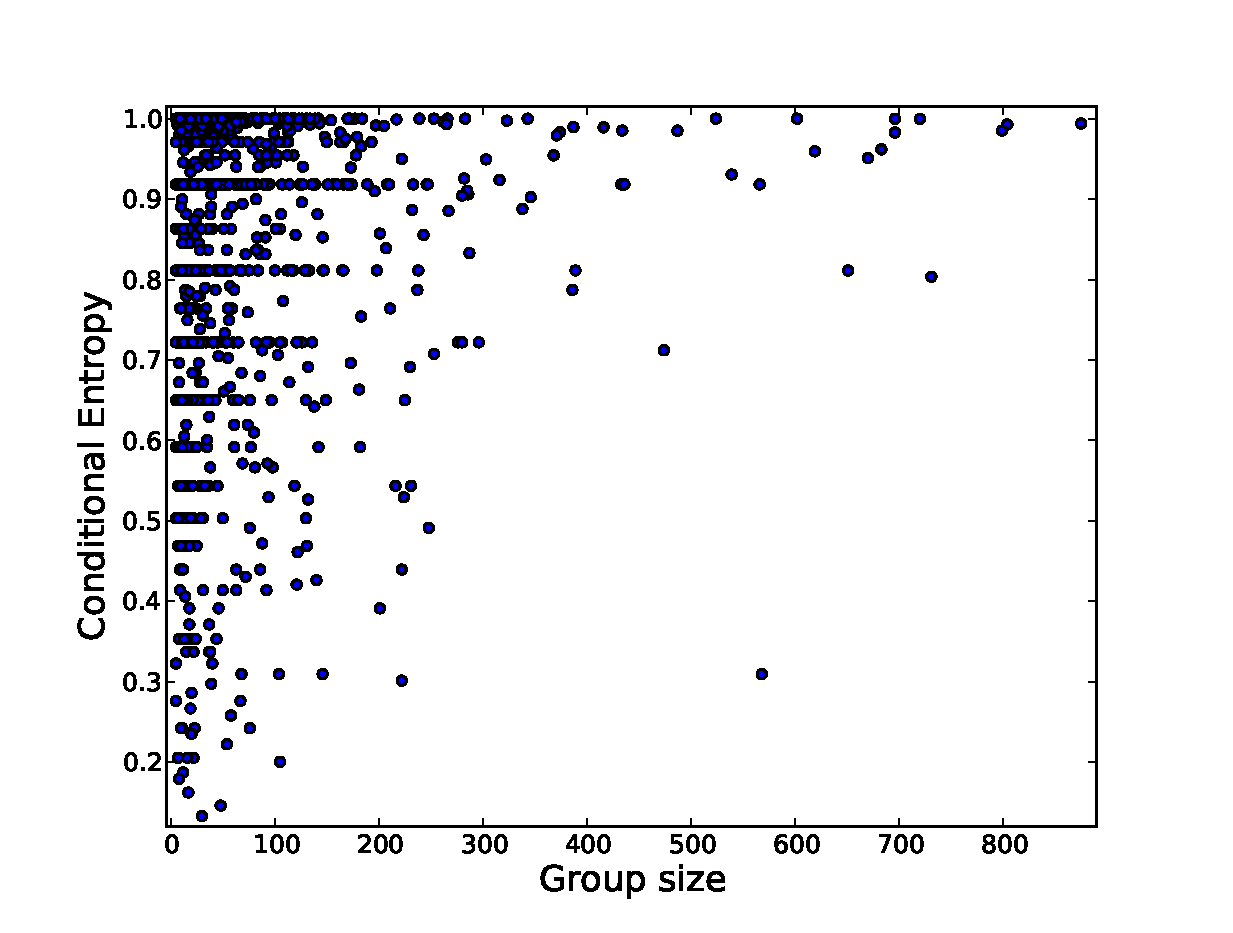
\includegraphics[width=45mm, height=35mm]{data/plots/new/CEvsGroupSize.eps}}
\subfloat[Fig:][]{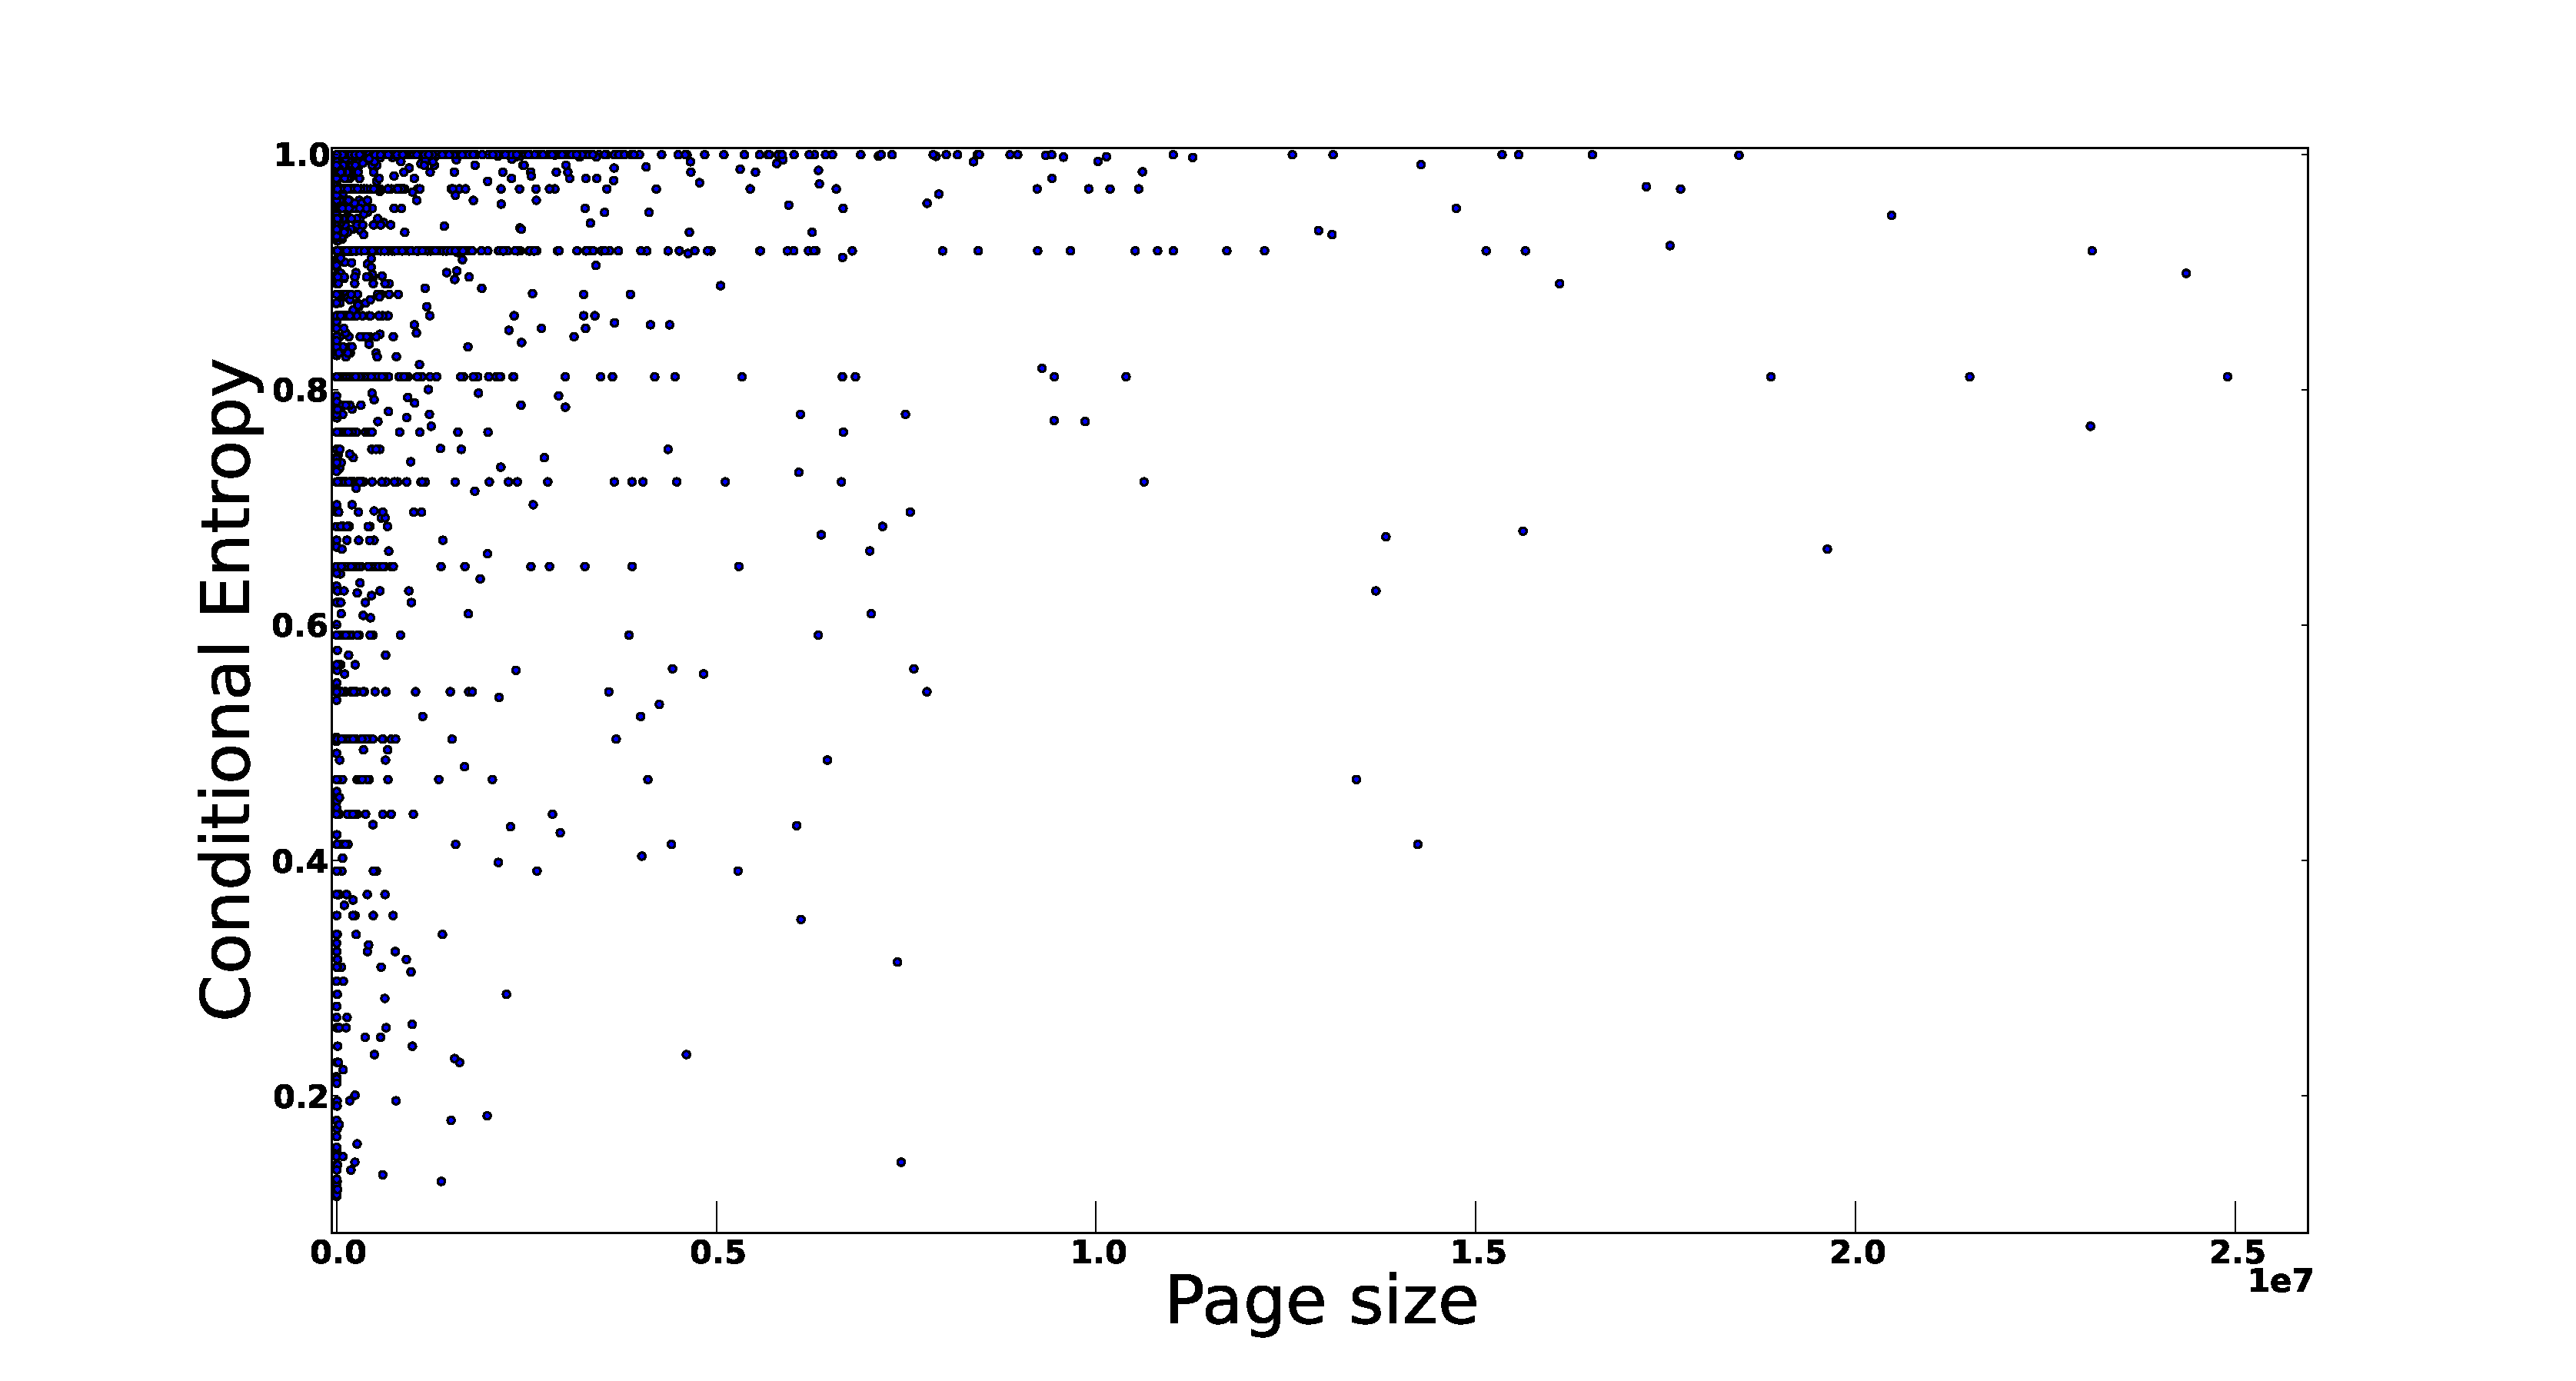
\includegraphics[width=45mm, height=35mm]{data/plots/new/CEvsPageSize.eps}}
\subfloat[Fig:][]{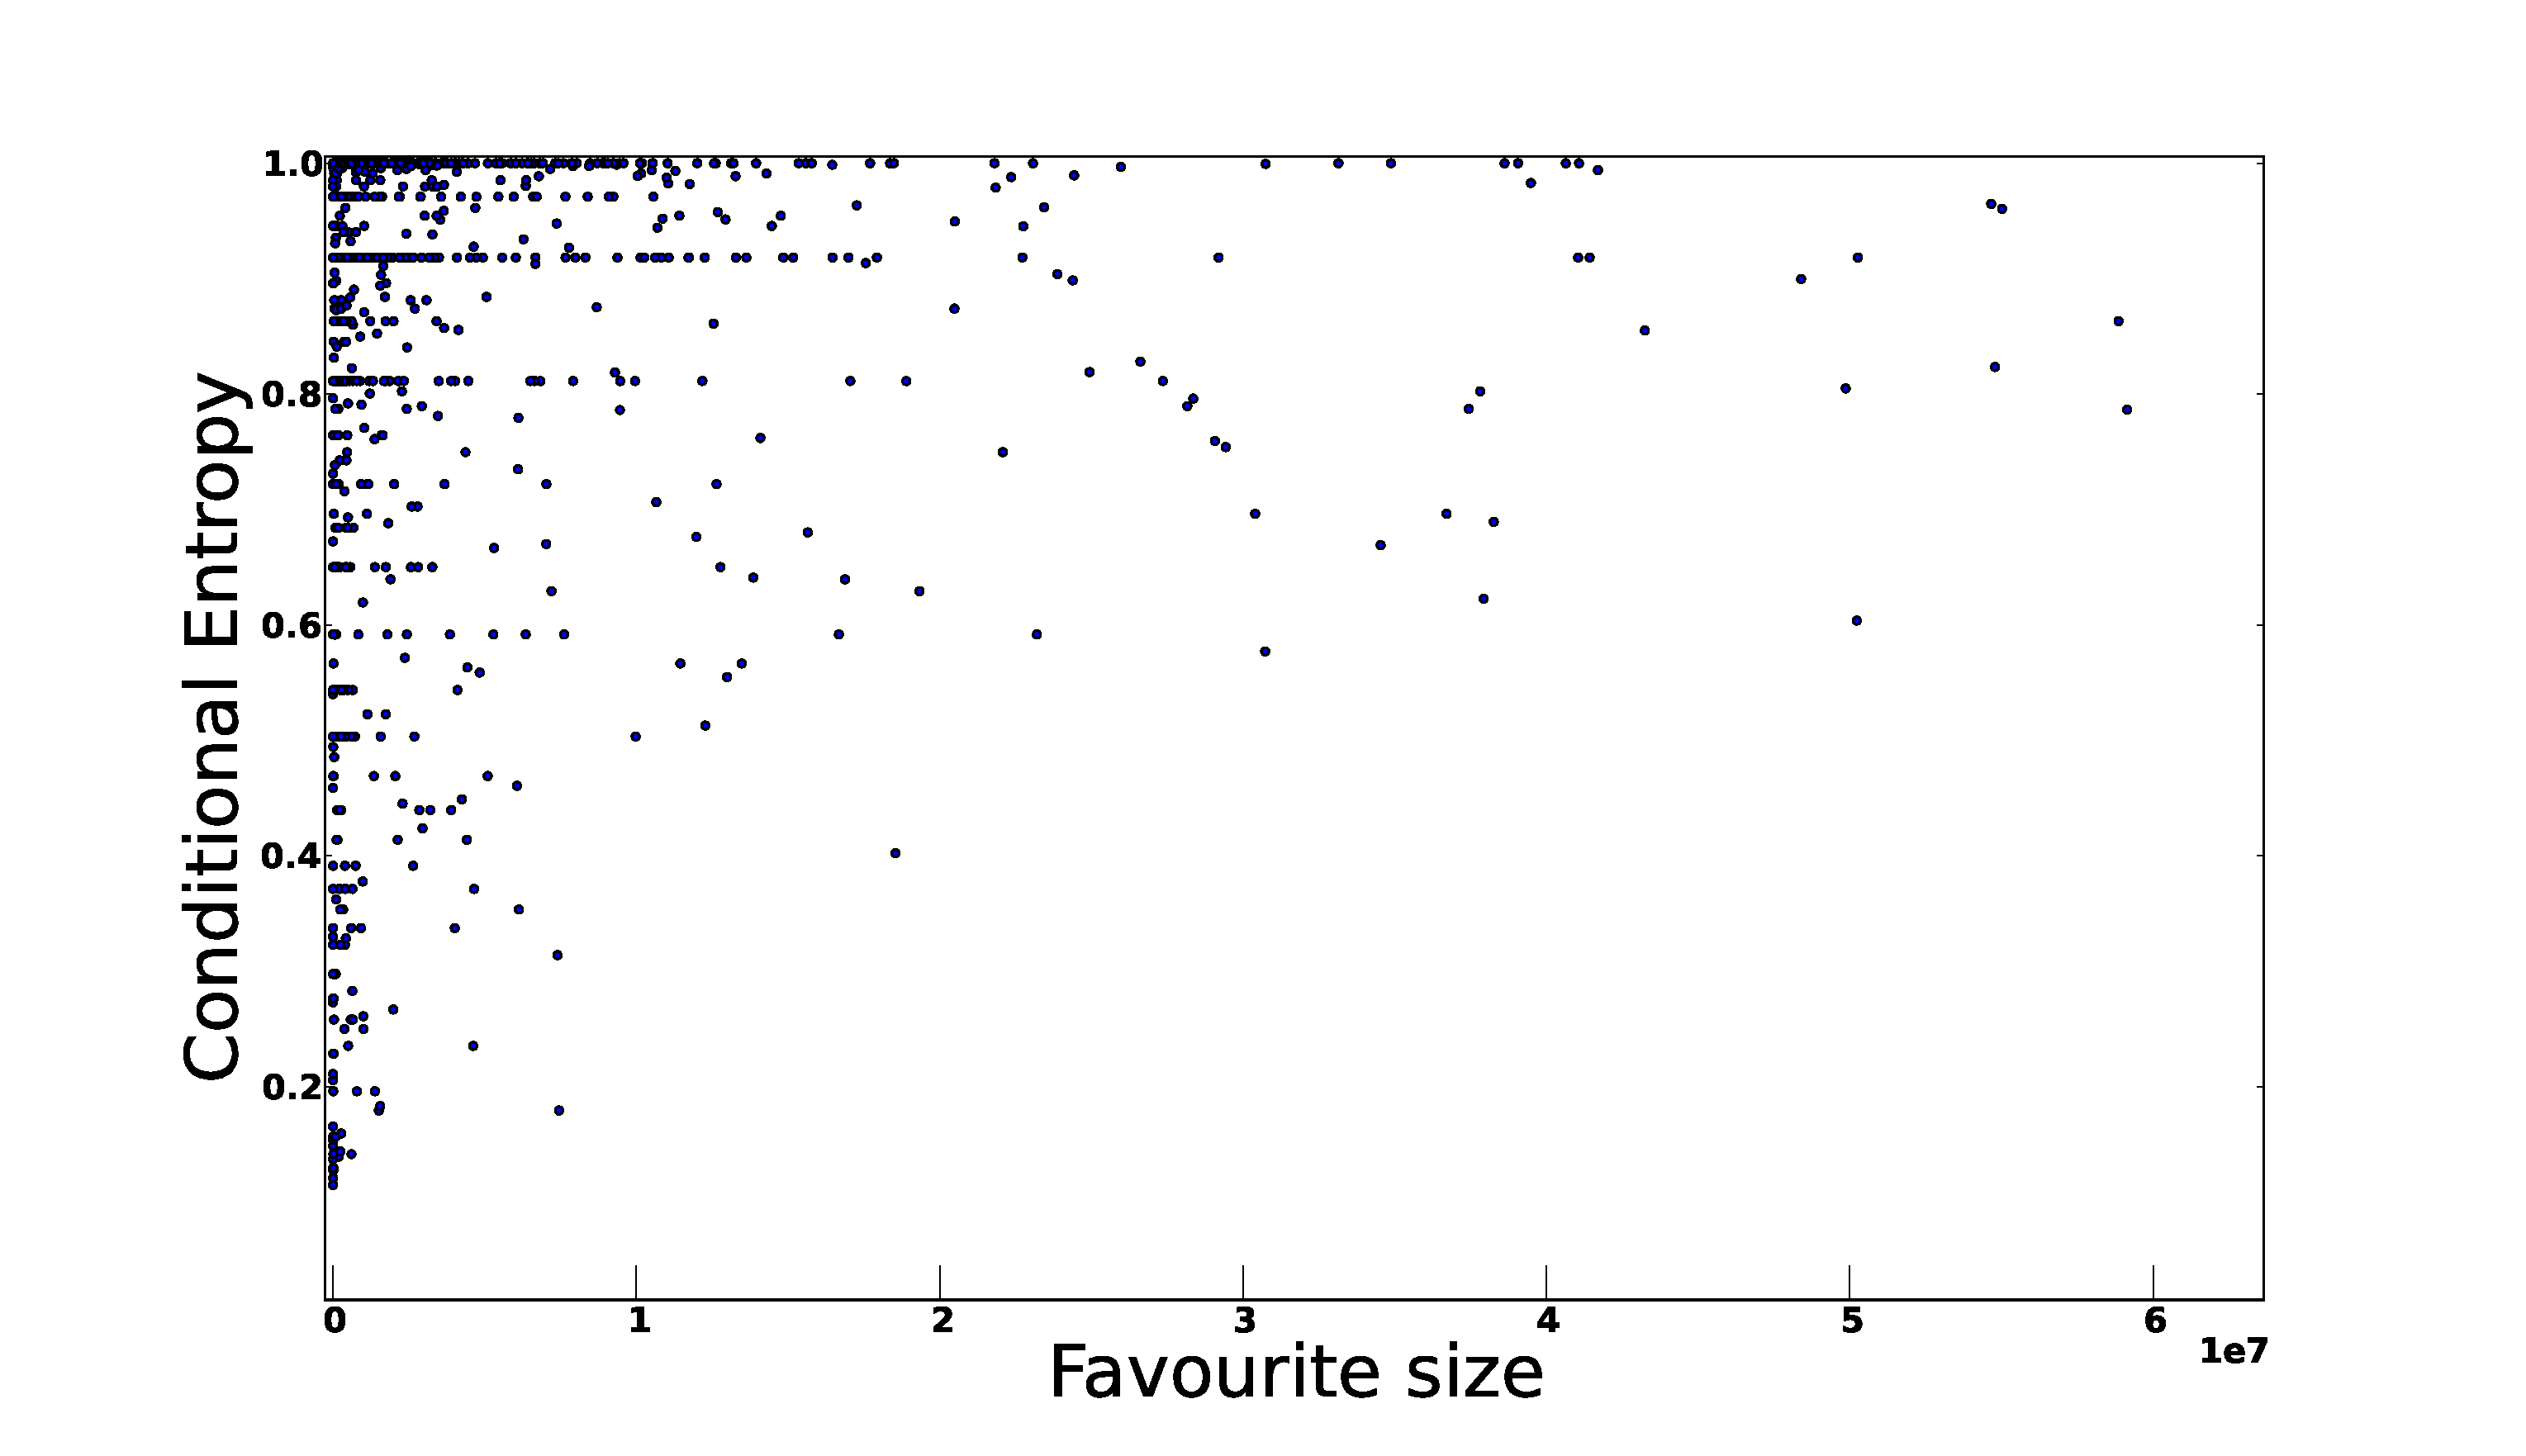
\includegraphics[width=45mm, height=35mm]{data/plots/new/CEvsFavSize.eps}} \\
%\vspace{-10mm}
\subfloat[Fig:][]{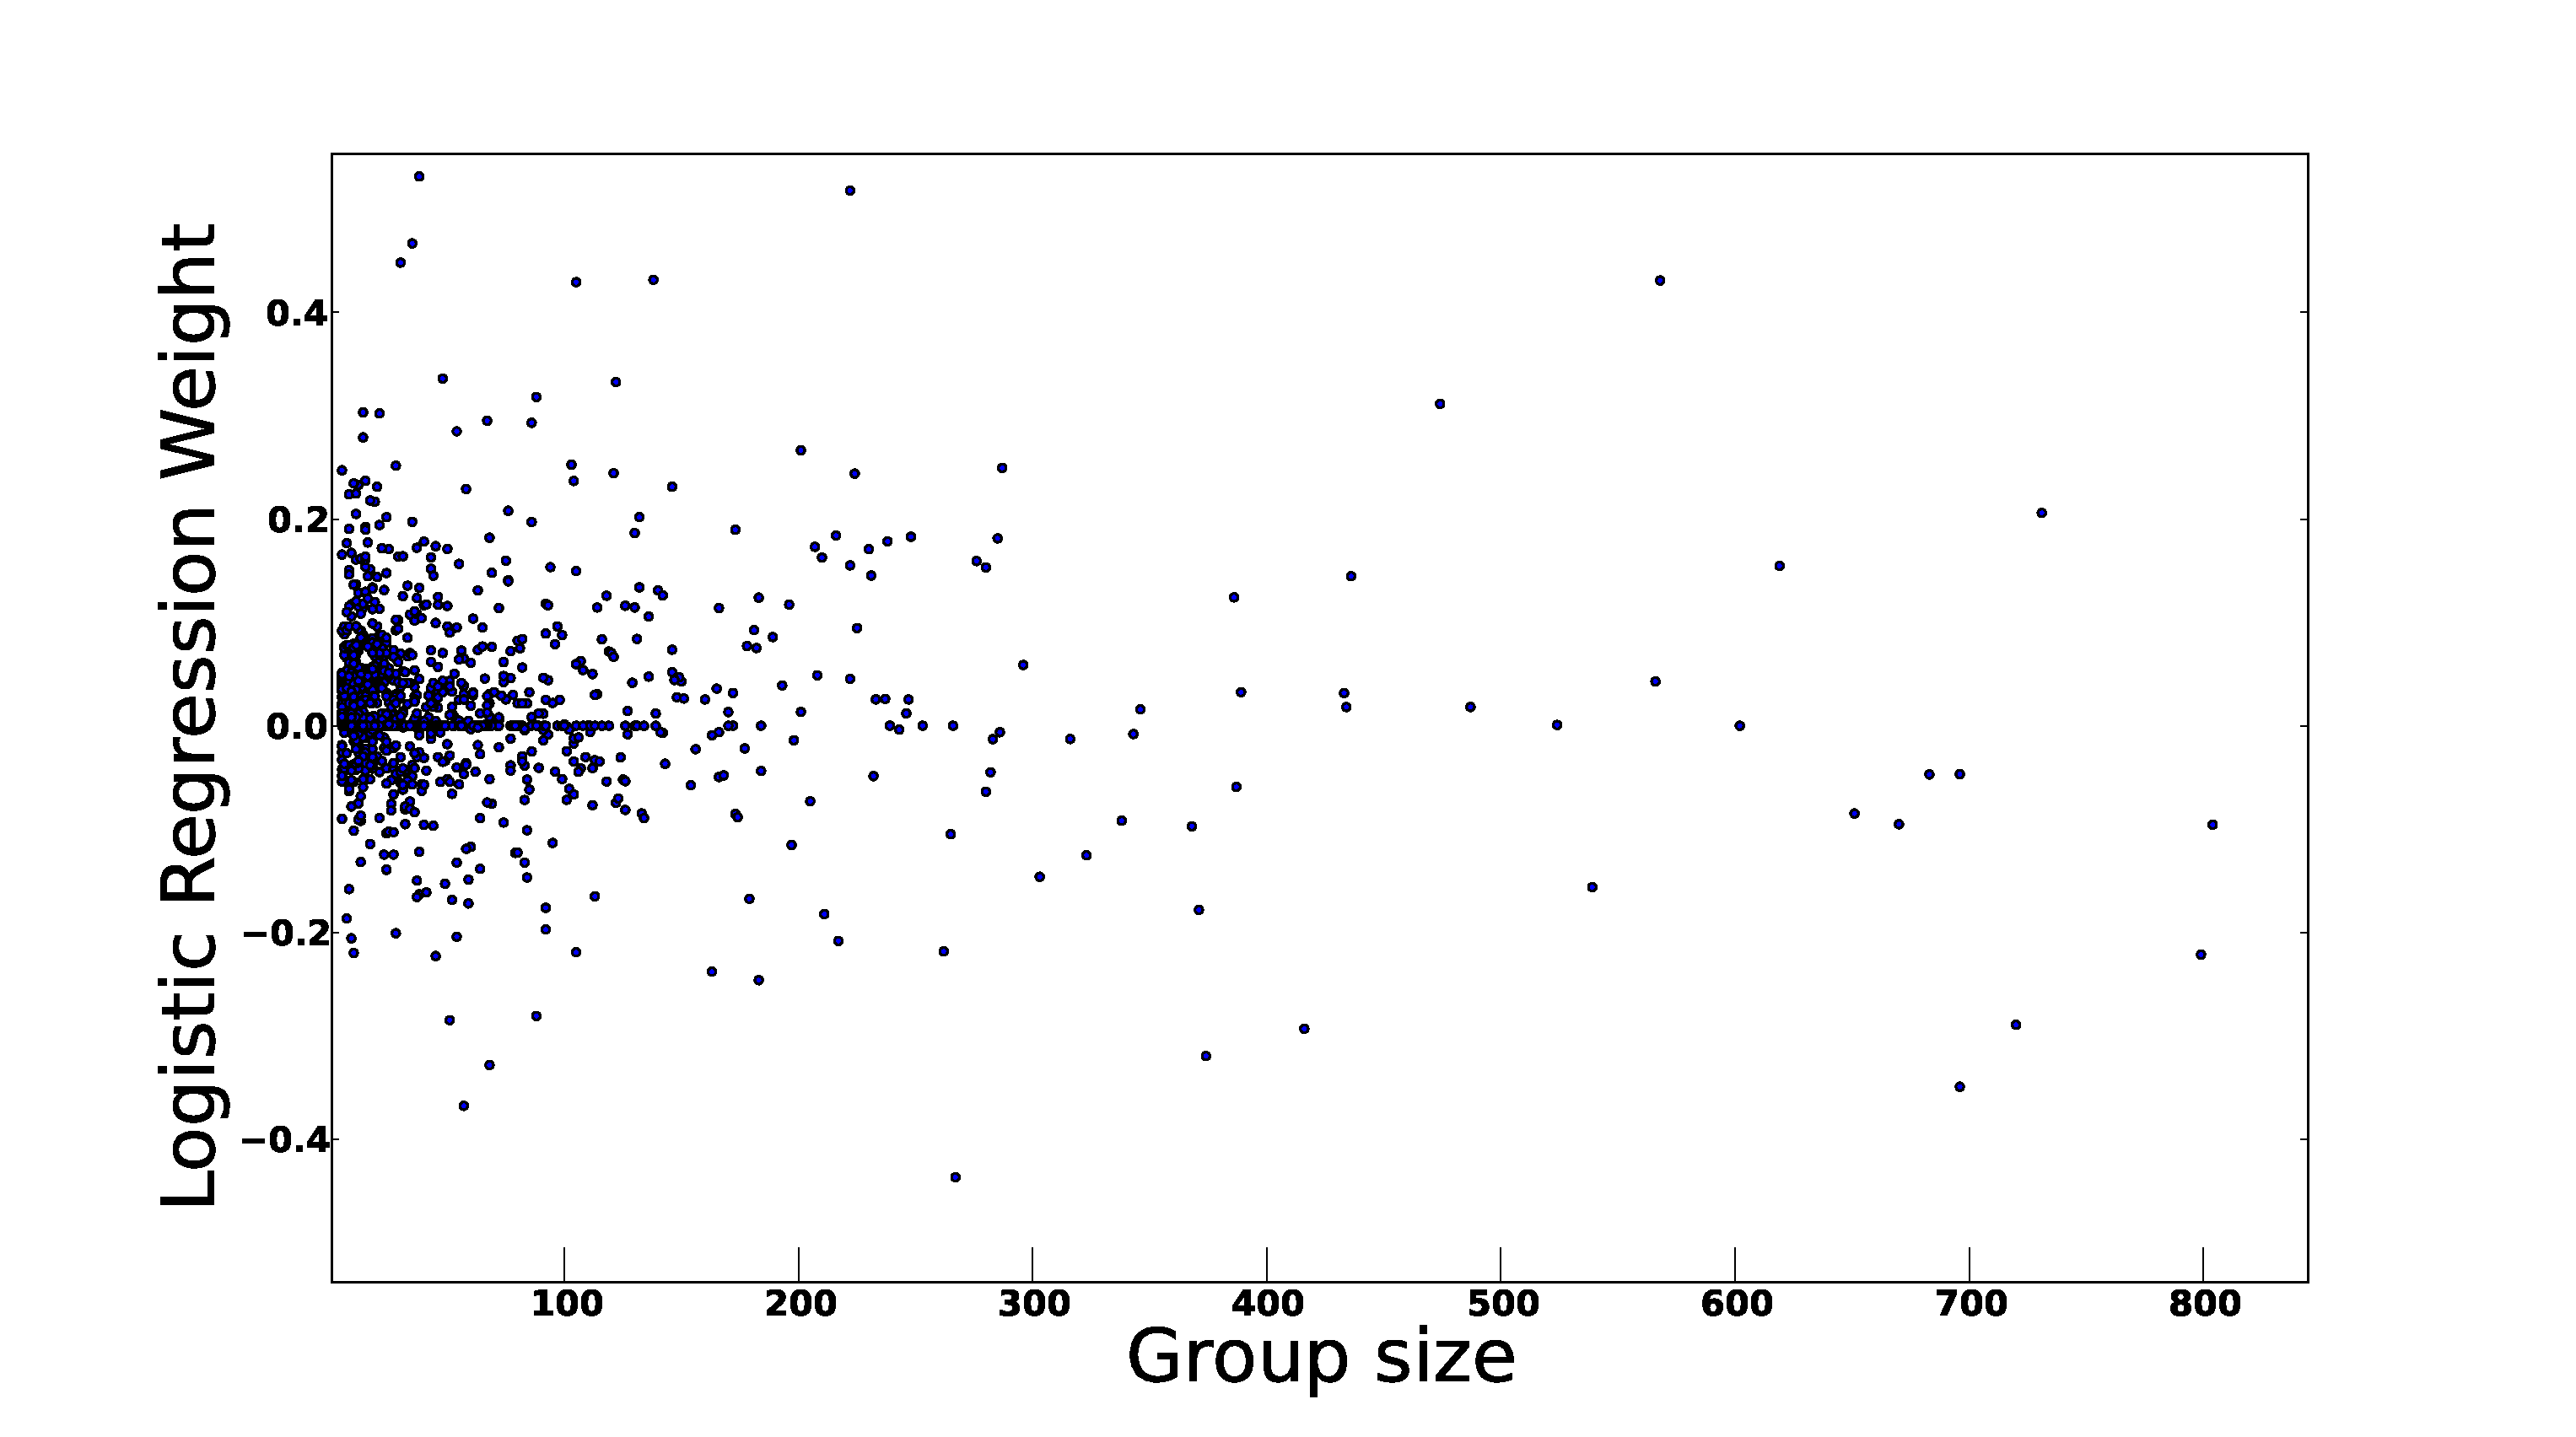
\includegraphics[width=45mm, height=35mm]{data/plots/new/LRweightvsGroupSize.eps}}
\subfloat[Fig:][]{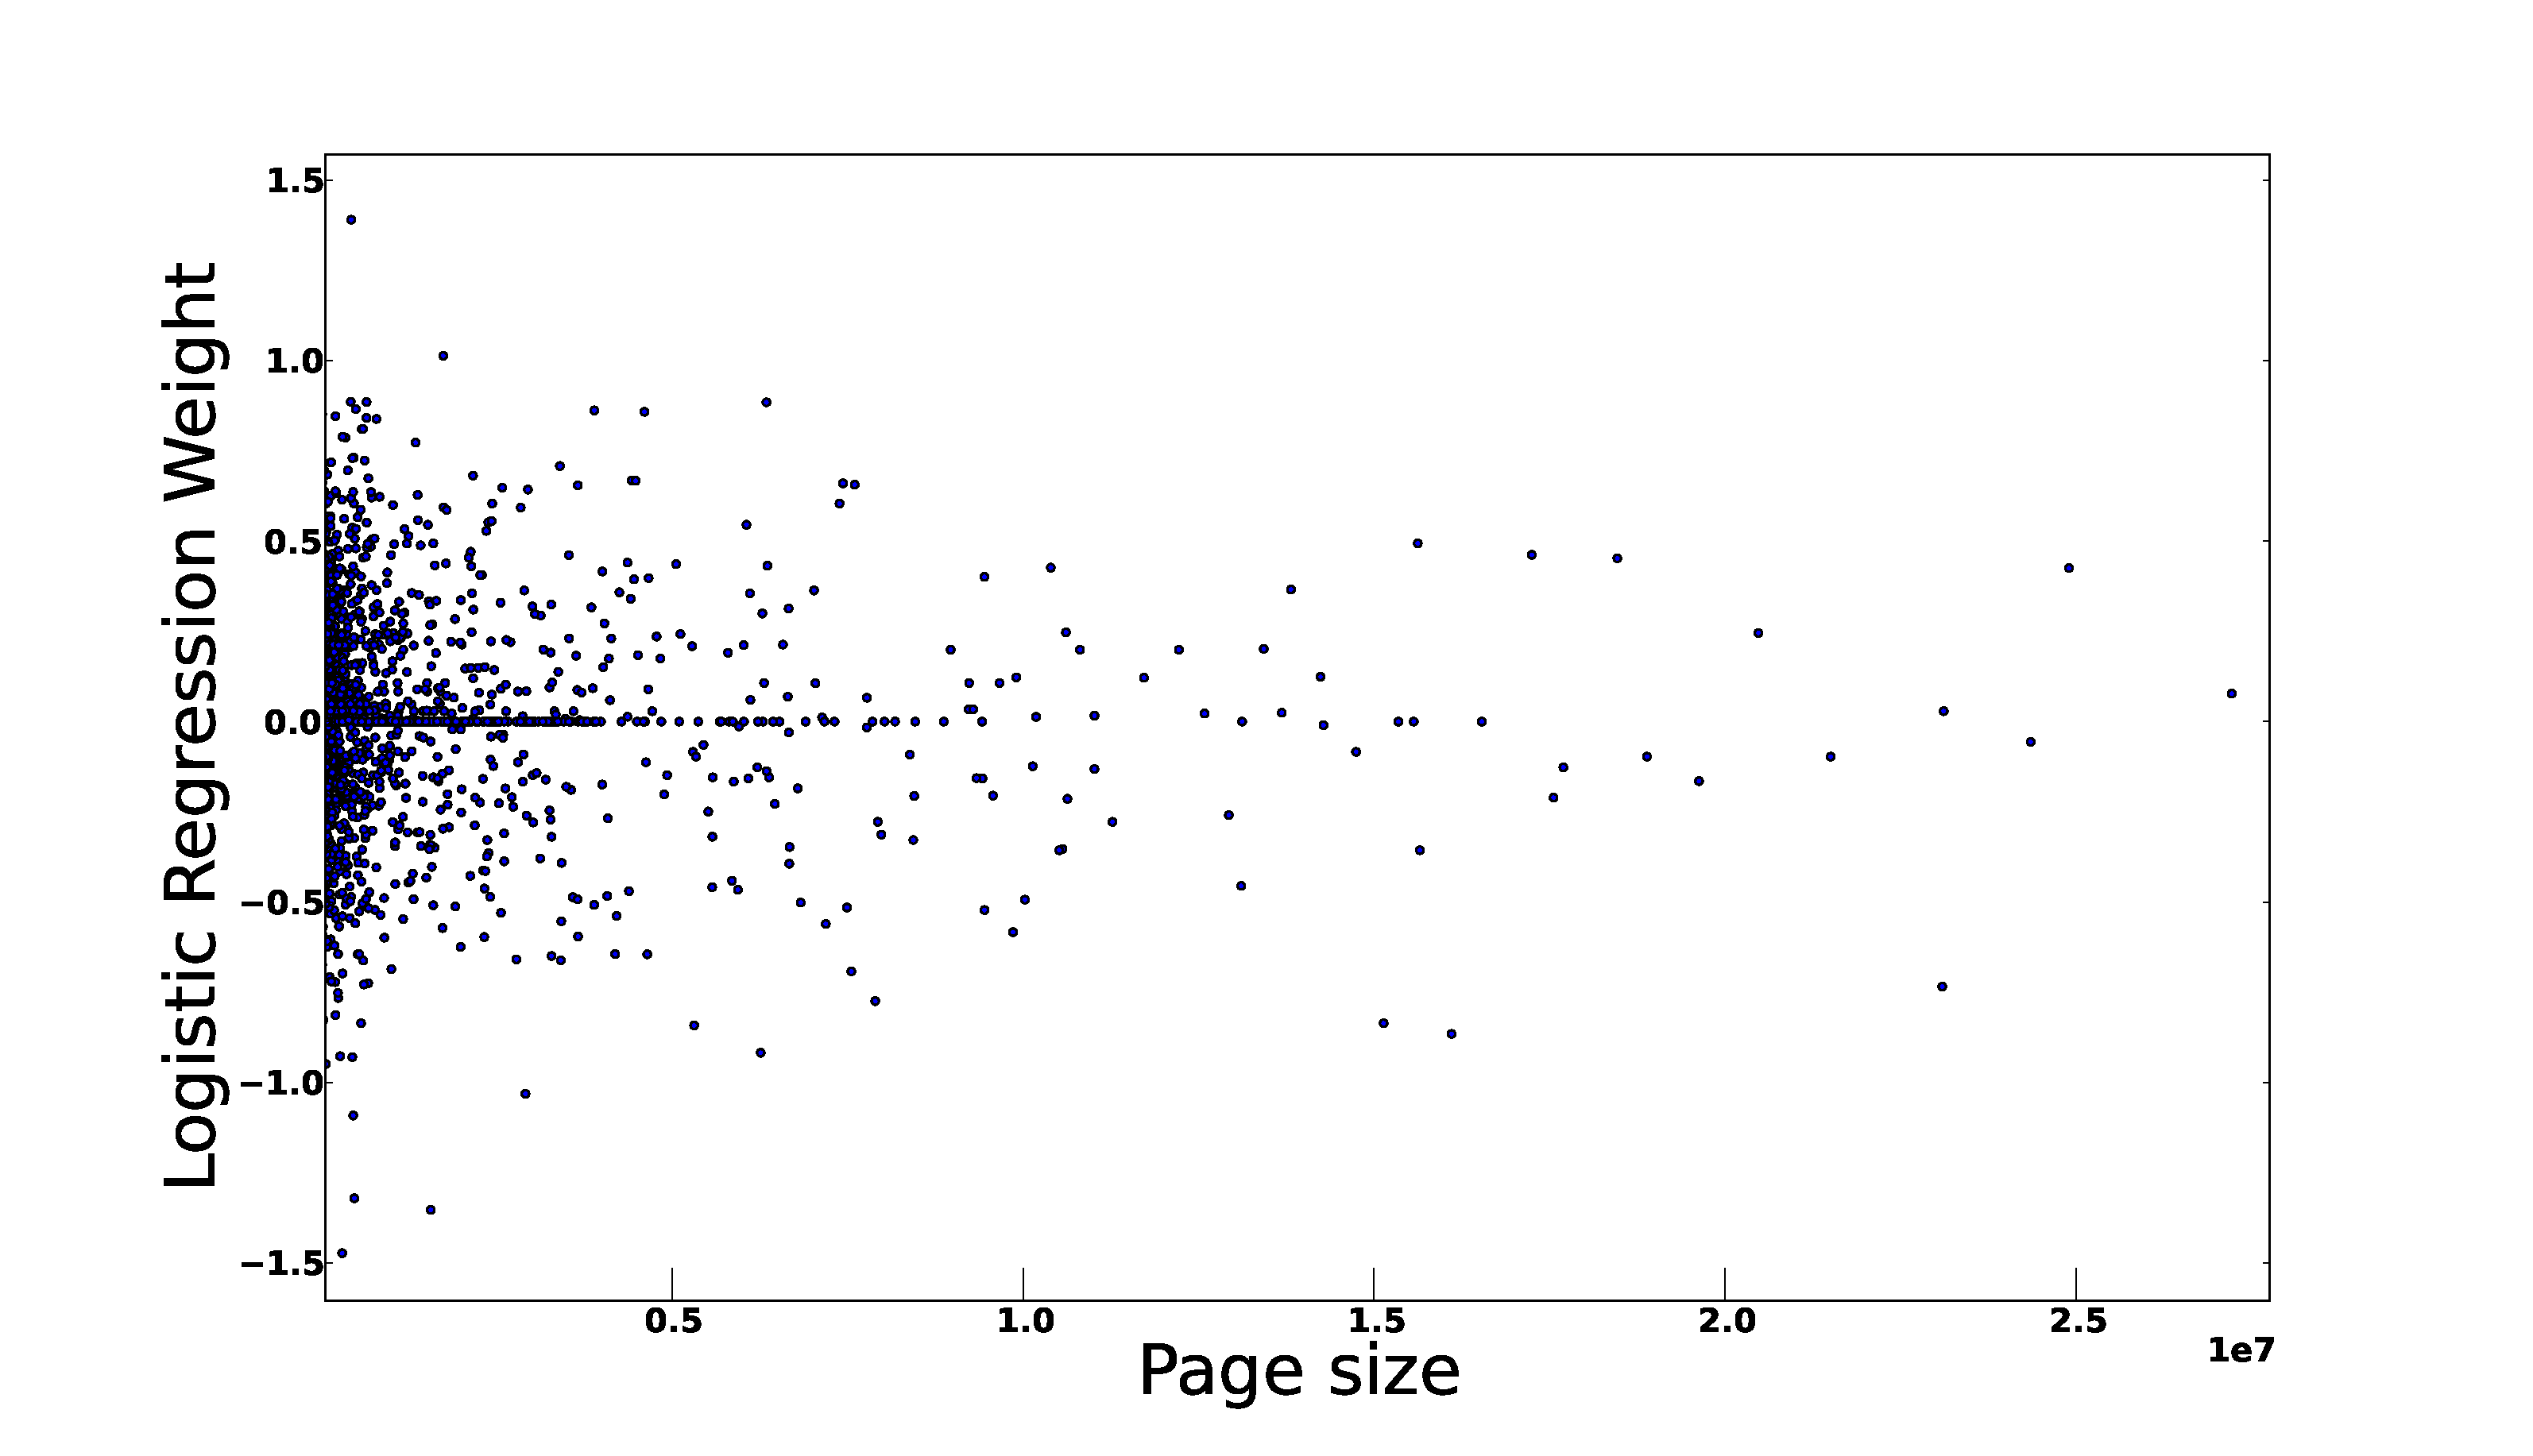
\includegraphics[width=45mm, height=35mm]{data/plots/new/LRweightvsPageSize.eps}}
\subfloat[Fig:][]{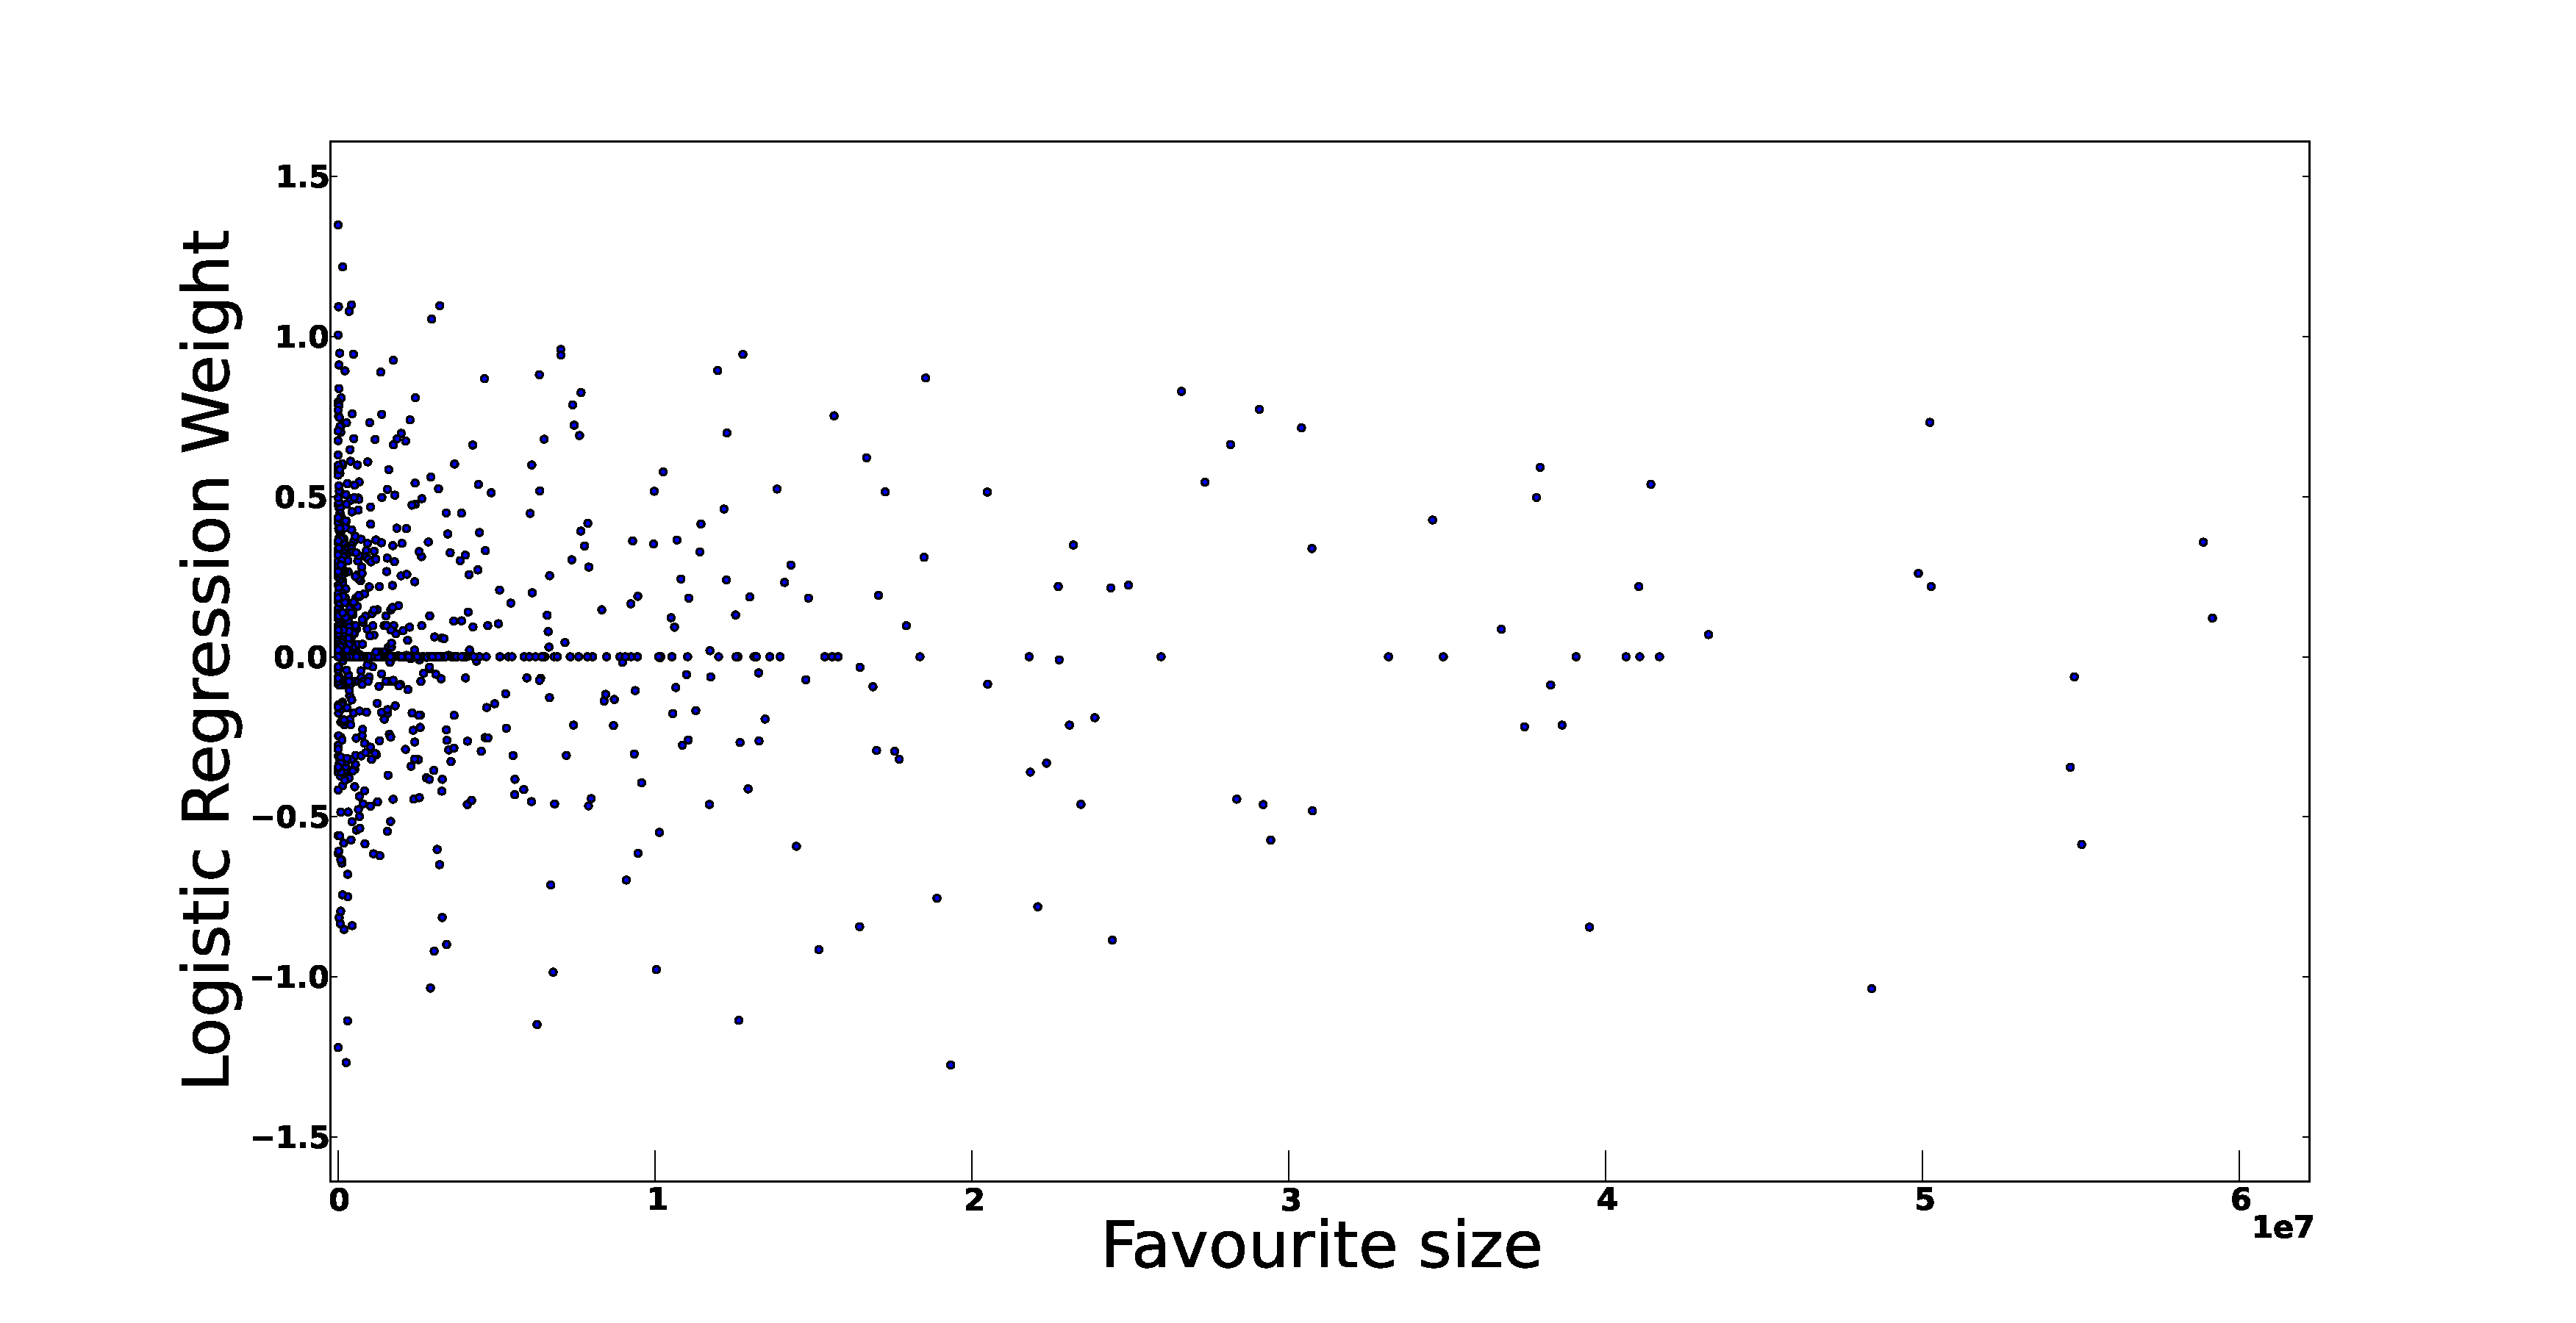
\includegraphics[width=45mm, height=35mm]{data/plots/new/LRweightvsFavSize.eps}} \\
\end{tabular}
\end{tabular}
\vspace{-2mm}
\caption {Conditional entropy vs. size (a-c); logistic regression feature weights vs size (d-f).
In (a-c) we observe that the large membership ASAGs are rarely
informative while the most informative SAGs tend to have low
memberships.  Similarly in (d-f) we see that the most predictive
features with the largest weights (positive or negative) are
concentrated toward small ASAGs. }
\label{Fig3}
\end{figure*}
%%%%%%%%%%%%%%%%%%%%%%%%%%%%%%%%%%%%%%%%%%%%%%%%%%%%%%%%%%%%%%%%%%%%%%%%%%%

%\vspace{-5mm}

%%%%%%%%%%%%%%%%%%%%%%%%%%%%%%%%%%%%%%%%%%%%%%%%%%%%%%%%%%%%%%%%%%%%%%%%%%%
\begin{figure*}[tbph!]
\centering
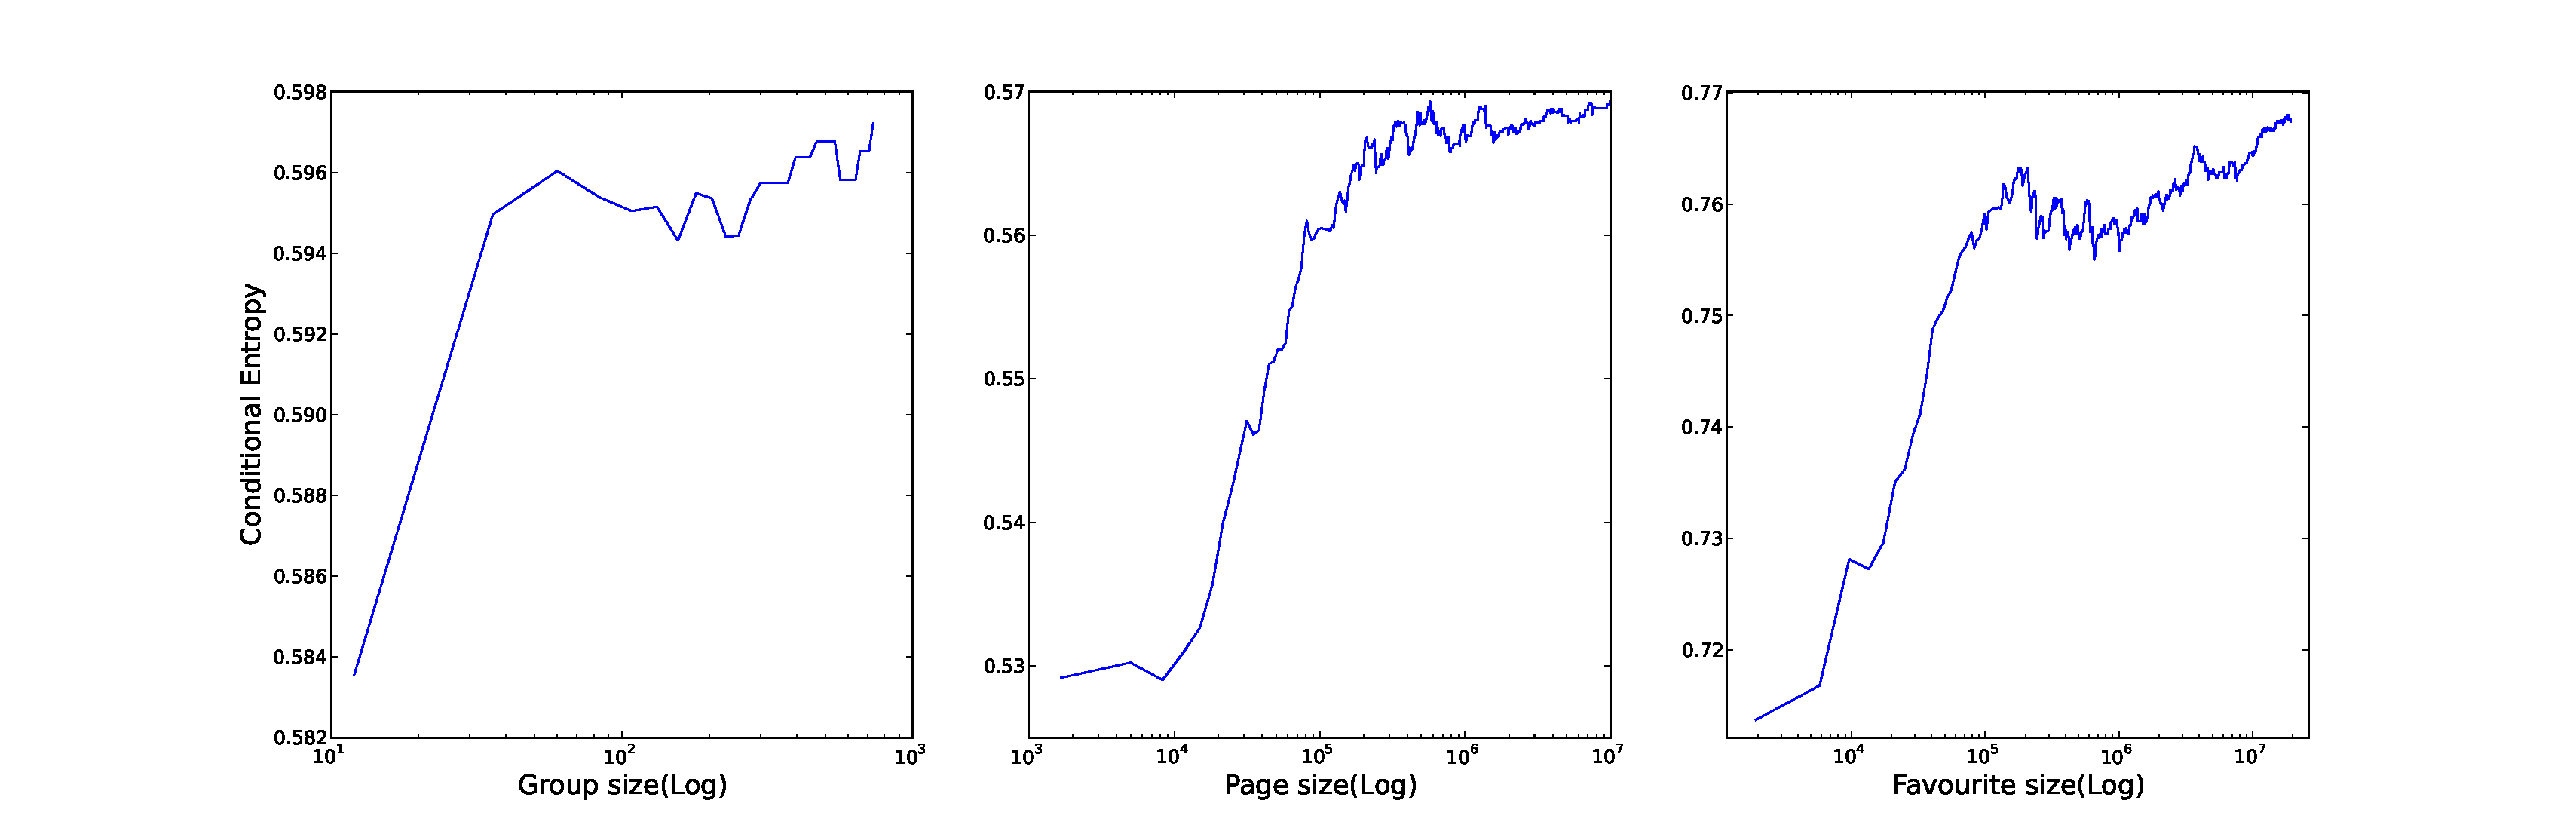
\includegraphics[scale=0.28]{data/plots/cumulativeEntropy/cumulative.eps}
\vspace{-3mm}
\caption{Average conditional entropy of top 10\% groups, pages and favourite features \emph{cumulative} over the size.  Here we see that as we add in larger membership ASAGs, the average informativeness
decreases substantially (entropy increases).}
\label{Fig4}
\end{figure*}
%%%%%%%%%%%%%%%%%%%%%%%%%%%%%%%%%%%%%%%%%%%%%%%%%%%%%%%%%%%%%%%%%%%%%%%%%%%

%\vspace{-7mm}

%%%%%%%%%%%%%%%%%%%%%%%%%%%%%%%%%%%%%%%%%%%%%%%%%%%%%%%%%%%%%%%%%%%%%%%%%%%
\begin{figure*}[tbph!]
\hspace{-12mm}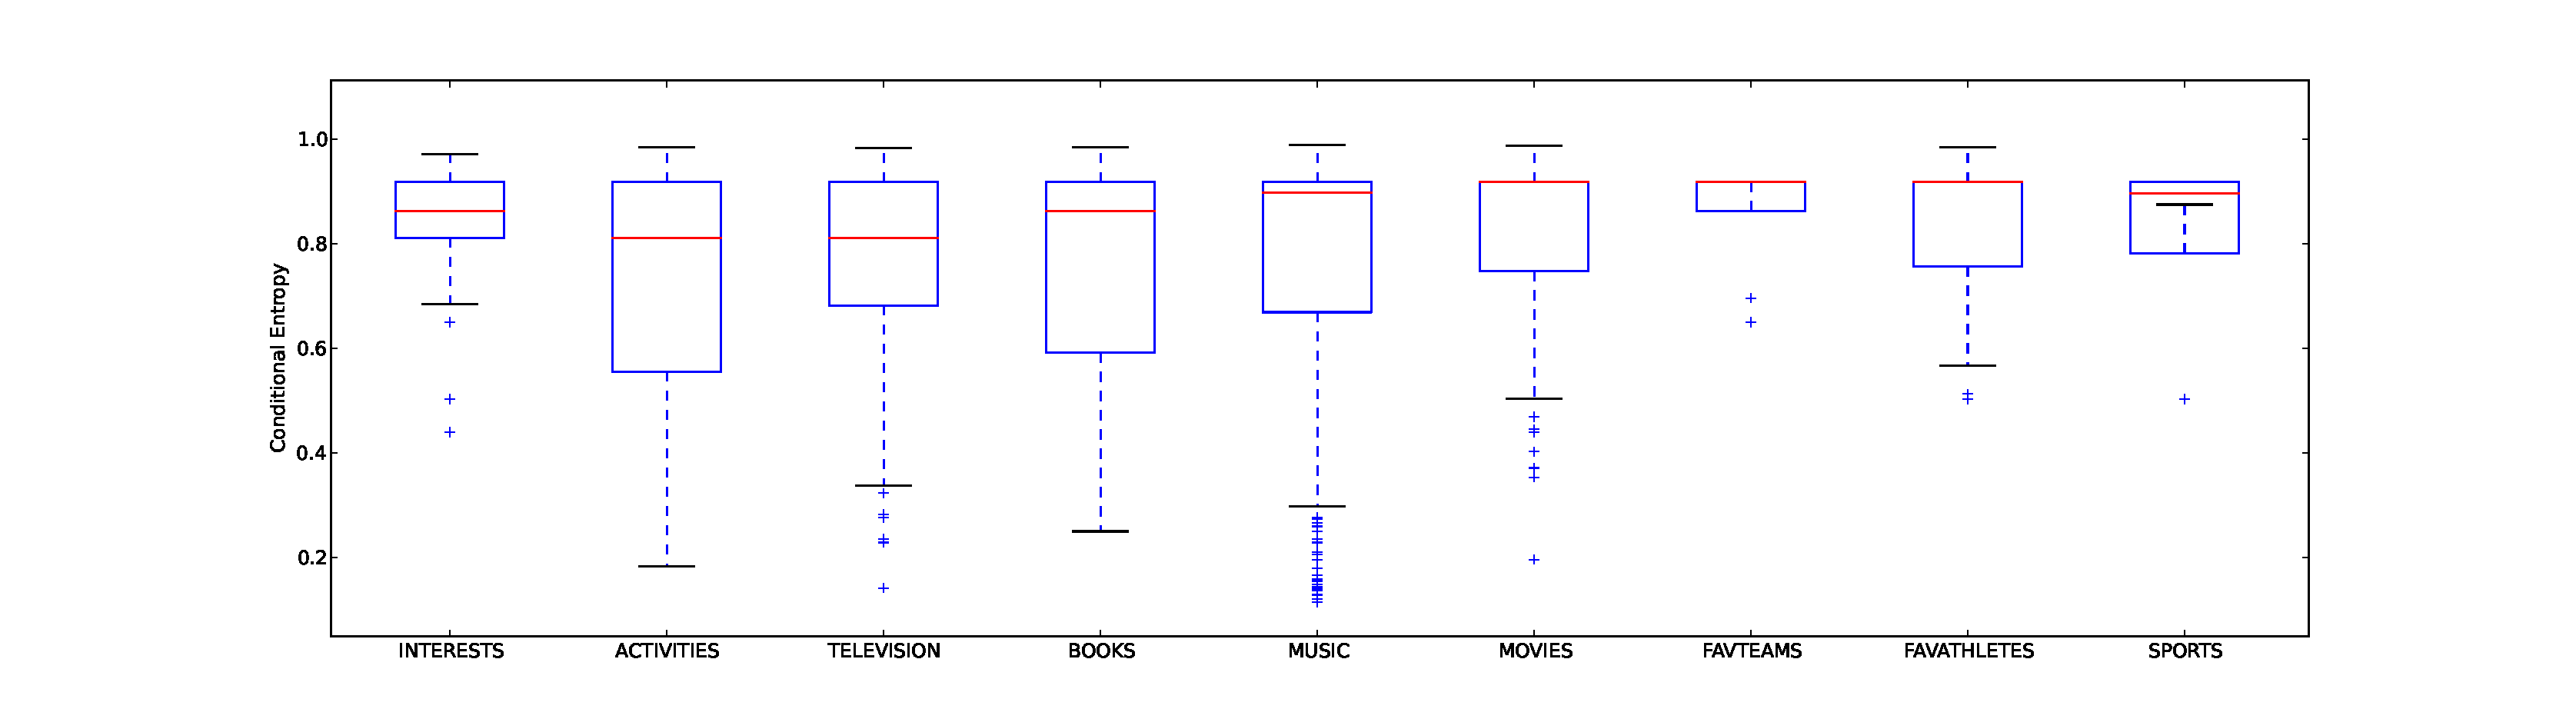
\includegraphics[width=200mm]{data/plots/boxPlots/CEvsFavTypes.eps}
\vspace{-7mm}
\caption{Conditional entropy for top 1000 favourites breakdown by categories.  While
at least half of ASAG categories
with many options like music are not informative (judging by median values), 
some of the most informative ASAGs are music.  This reiterates
the point that it is crucial to \emph{learn} which ASAGs 
are informative rather than aggregating average information.}
\label{Fig5}
\end{figure*}
%%%%%%%%%%%%%%%%%%%%%%%%%%%%%%%%%%%%%%%%%%%%%%%%%%%%%%%%%%%%%%%%%%%%%%%%%%%

%#suvash#

%%%%%%%%%%%%%%%%%%%%%%%%%%%%%%%%%%%%%%%%%%%%%%%%%%%%%%%%%%%%%%%%%%%%%%%%%%%
\begin{figure*}[tbh!]
\centering
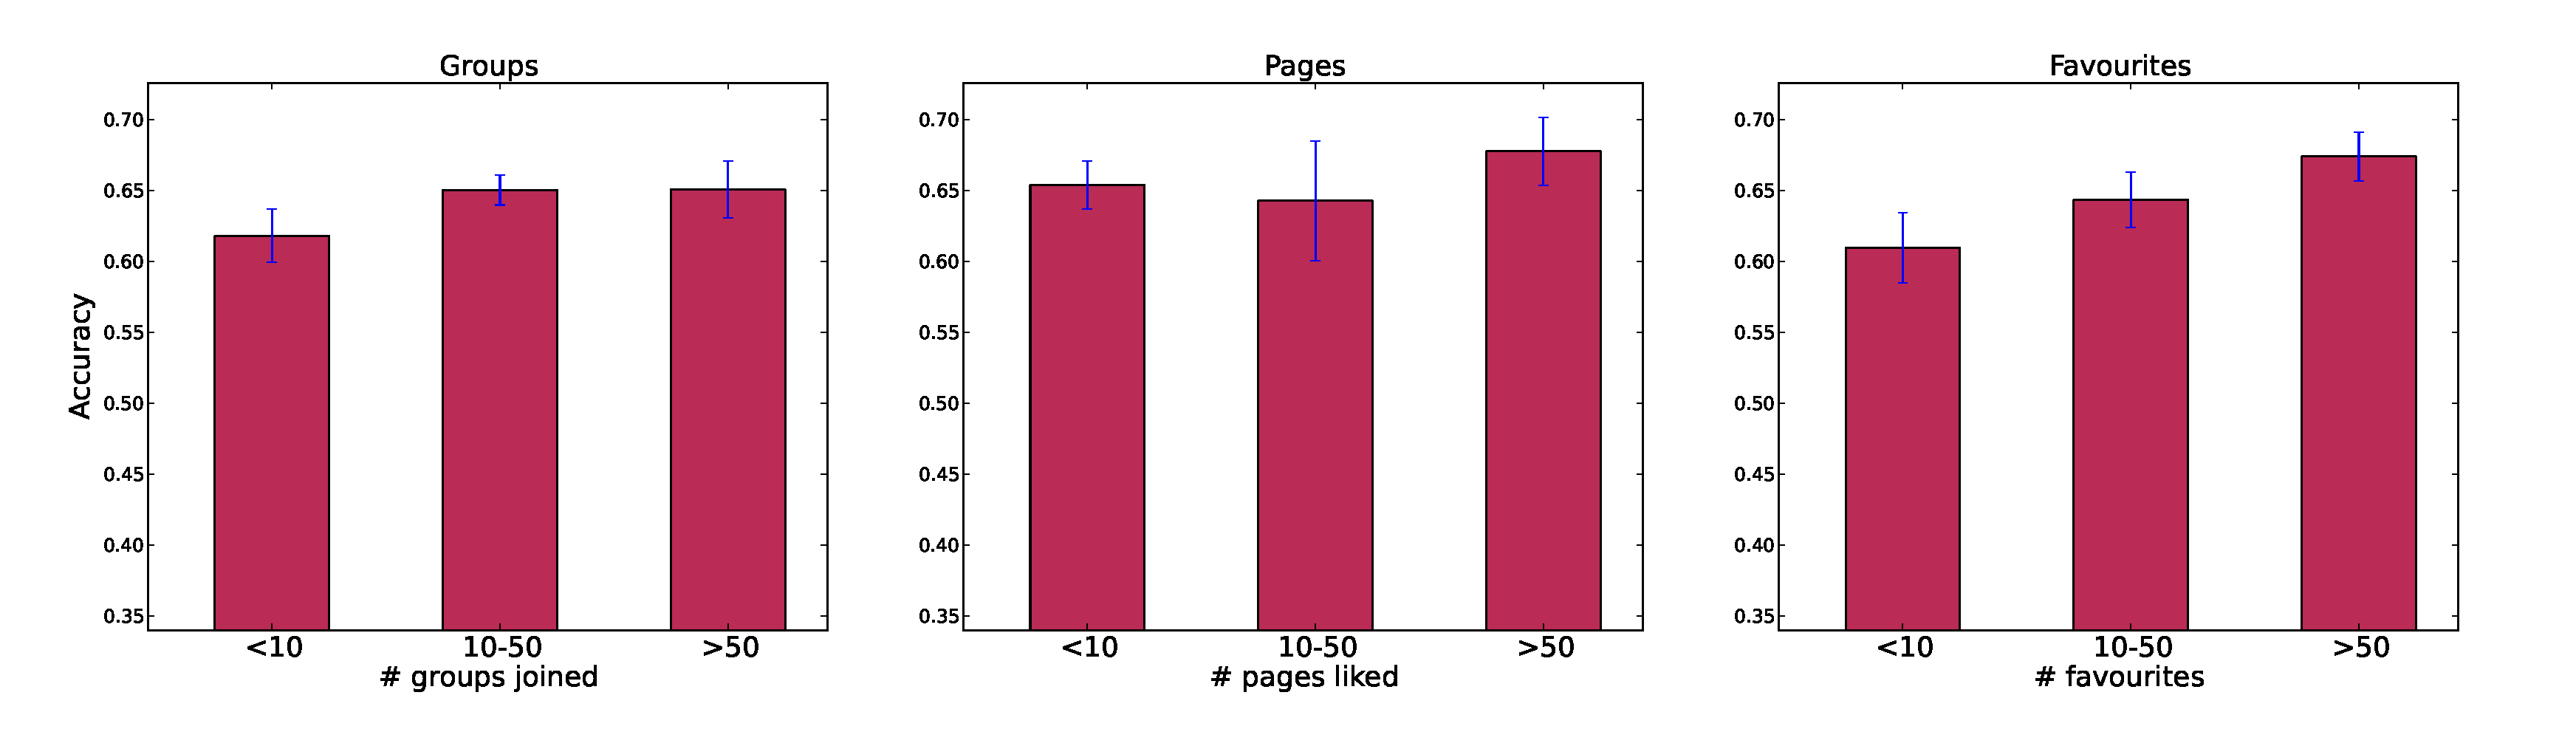
\includegraphics[width=180mm, height=50mm]{data/plots/new/accuracyVsmembership.eps}
\vspace{-6mm}
\caption{Accuracy of the SAF increases as users become more active in social network by joining more groups/pages/favourites.  It does not appear too many activities hurts --- SAF learns to discriminate when activities are predctive.}
\label{AccuracyVsmembership}
\end{figure*}
%%%%%%%%%%%%%%%%%%%%%%%%%%%%%%%%%%%%%%%%%%%%%%%%%%%%%%%%%%%%%%%%%%%%%%%%%%%

%%%%%%%%%%%%%%%%%%%%%%%%%%%%%%%%%%%%%%%%%%%%%%%%%%%%%%%%%%%%%%%%%%%%%%%%%%%
\begin{figure*}[tbh!]
\centering
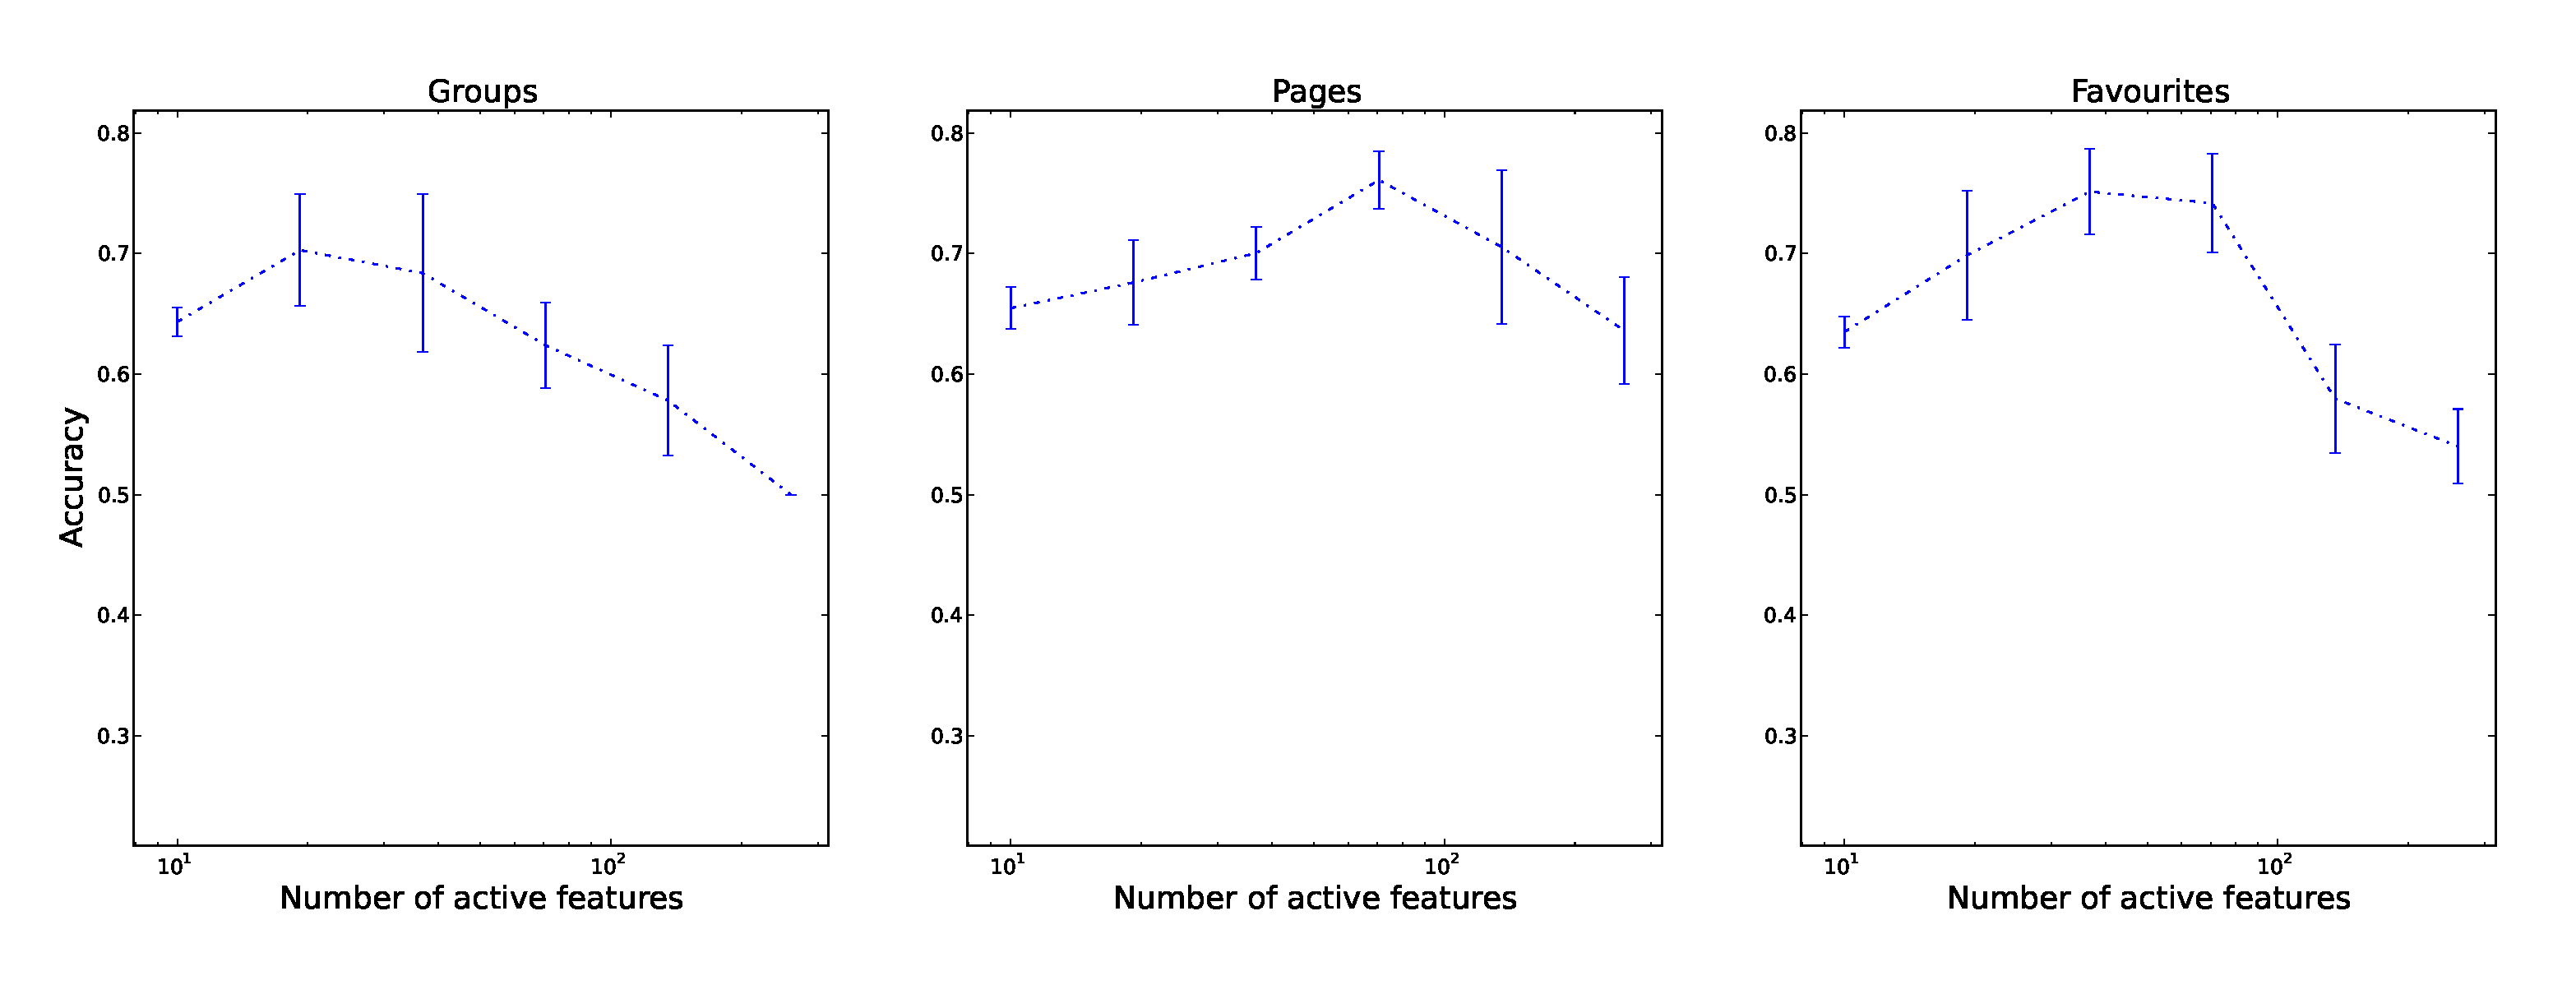
\includegraphics[width=180mm, height=50mm]{data/plots/new/accuracyVsactiveFeatures.eps}
\vspace{-6mm}
\caption{Accuracy increases as the number of active features increases, but then, after reaching a certain limit, it starts to decrease, i.e., excessive item popularity among activities hurts the discriminative power of SAF to make good recommendations.}
\label{fig:AccuracyVsactiveFeats}
\end{figure*}
%%%%%%%%%%%%%%%%%%%%%%%%%%%%%%%%%%%%%%%%%%%%%%%%%%%%%%%%%%%%%%%%%%%%%%%%%%%
